\chapter{Opdracht 4: Web API}
Onze applicatie presenteert zichzelf naar buiten toe via het web:
we reageren op HTTP requests en geven HTTP responses terug.

\subsection{Client/server-architectuur}
Het web werkt volgens een client/server-architectuur (of klant/bediende-model):
We hebben een client, bijvoorbeeld een web browser, die een verzoek doet 
aan een server die dit afhandelt. Zie Figuur~\ref{fig:client-server}.

\begin{figure}[H]
    \centering
    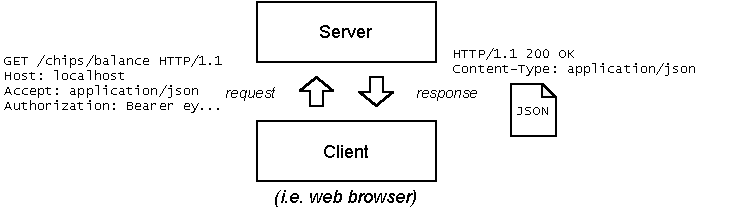
\includegraphics[width=.9\linewidth]{client-server}
    \caption{HTTP requests worden van een client gestuurd naar een server, welke dit verwerkt en reageert met een HTTP response.}
    \label{fig:client-server}
\end{figure}

\subsection{Content negotiation}
Zoals in Figuur~\ref{fig:client-server} is te zien, 
onderhandelen client en server over het ophalen van een \textit{representatie}
van een bepaalde \textit{resource}. We zien dat de client een 
GET-verzoek doet naar localhost voor een Balance-resource te
vinden via de Uniform Resource Locator (URL) `chips/balance'
(in combinatie met de token in de Authorization header)
De gewenste representatie daarvan moet `application/json' zijn.

Deze interactie tussen client en server noem je \texit{content negotation}:
er is een scheiding tussen de abstractie en de verschijningsvorm ervan.

\subsection{HTTP requests}
Een HTTP request (zie Figuur~\ref{fig:client-server}) wordt gevormd door:
\begin{enumerate}
    \item Een beschrijving van method, URI en protocol
    \item Headers
    \item Optioneel: een request body met een representatie volgens Content-Type
\end{enumerate}

\subsubsection{HTTP methods}
De HTTP-specificatie beschrijft een aantal methodes 
waarmee een client allerlei zaken kan vragen aan een server.
Het is belangrijk om de juiste HTTP-methodes te gebruiken omdat 
deze in de eerste plaats het soort actie aangeven die wordt verzocht.

In de tweede plaats staat in de protocol-specificatie van HTTP heel 
nauwkeurig beschreven wat clients en servers mogen verwachten van een 
bepaalde HTTP-methodes. 
Twee van de te verwachten eigenschappen zijn \textit{safety}
en \textit{idempotentie}.

Een HTTP-method wordt als \textit{safe} beschouwt als deze niet 
de intentie heeft om de servertoestand aan te passen. 
Dat betekent dat het gaat om read-only methoden. Safe 
methoden kunnen helpen bij het cachen van resultaten (zie: REST).
Bij safety gaat het dus niet om de beveiliging, het ziet 
erop dat het veilig is omdat het geen toestand kan aanpassen.

Wanneer een HTTP-method \textit{idempotent} wordt genoemd,
betekent dat dat we het verzoek meerdere keren kunnen herhalen
zonder dat de uitkomst op server verandert. Denk bijvoorbeeld aan 
het tweemaal uitvoeren van een \texttt{DELETE}-methode. Beide keren is 
de betreffende resource verwijderd. Idempotentie helpt een API betrouwbaar 
te maken tegen fouten: het betekent dat je een verzoek kan herhalen zonder 
als je als client niet zeker weet of het is aangekomen of niet.

We kennen de volgende HTTP-methods, zie Figuur~\ref{table:http-methods}:

\begin{table}[H]
\centering
\begin{tabularx}{\textwidth}{|>{\raggedright}l|>{\raggedright}l|>{\raggedright\arraybackslash}X|}
\hline
\textbf{HTTP-method} & \textbf{Bedoeling} & \textbf{Safe} & \textbf{Idempotent} \\ \hline
\texttt{GET} & opvragen van resource(s) & Ja & Ja \\ \hline
\texttt{HEAD} & opvragen van headers (voordat je een mogelijk grote GET-request doet) & Ja & Ja \\ \hline
\texttt{OPTIONS} & opvragen van toegestane communicatiewijzen voor een bepaalde URL of server & Ja & Ja \\ \hline
\texttt{TRACE} & opvragen van afgelegde weg van het verzoek ter debugging & Ja & Ja \\ \hline
\texttt{DELETE} & verwijderen van gehele resource op basis van URL (met identifier) & Nee & Ja \\ \hline
\texttt{PUT} & aanmaken/wijzigen van gehele resource op basis van URL (met identifier) & Nee & Ja \\ \hline
\texttt{PATCH} & wijzigen van deel van resource op basis van URL (met identifier) & Nee & Nee \\ \hline
\texttt{POST} & aanmaken nieuwe resource op onder een bepaalde URL (zonder identifier) & Nee & Nee \\ \hline
\end{tabularx}
\caption{Een opsomming van HTTP-methoden, hun bedoeling en verwachte eigenschappen}
\label{table:http-methods}
\centering
\end{table}

\subsection{HTTP responses}
Een HTTP response (zie Figuur~\ref{fig:client-server}) wordt gevormd door:
\begin{enumerate}
    \item Een beschrijving van protocol en statuscode
    \item Headers
    \item Optioneel: response body met een representatie volgens Content-Type 
\end{enumerate}

\subsubsection{Status codes}
Het teruggeven van de juiste statuscode is erg belangrijk wanneer je een API 
ontwerpt. Het maakt een bepaalde verwachting duidelijk en clients krijgen zo 
de mogelijkheid om slim om te gaan als er bijvoorbeeld een redirection moet plaatsvinden
of als de client wat verkeerd heeft gedaan.

HTTP status codes worden onderverdeeld 5 categorieën, waarbij 
het eerste getal steeds de categorie aangeeft (we noemen er hier een paar):
\begin{itemize}
    \item \textbf{1xx Informational}: request ontvangen, verwerking gaat door
        \begin{itemize}
            \item \textbf{100 Continue}: wordt gebruikt als een client eerst wil checken of de server het verzoek 
            gaat accepteren, bijvoorbeeld bij grote request bodies.
        \end{itemize}
    \item \textbf{2xx Successful}: request ontvangen, begrepen, en geaccepteerd zonder problemen
        \begin{itemize}
            \item \textbf{200 OK}: standaardresponse voor succesvolle afhandeling
            \item \textbf{201 Created}: verzoek is afgehandeld; een resource is succesvol aangemaakt
            \item \textbf{202 Accepted}: verzoek is succesvol binnengekomen, maar de uitvoering volgt nog
        \end{itemize}
    \item \textbf{3xx Redirection}: meer actie is vereist om het verzoek af te handelen
    \begin{itemize}
        \item \textbf{303 See Other}: de response voor het request kan worden opgehaald (met GET) via de getoonde URI
        \item \textbf{307 Temporary Redirect}: dit verzoek, niet volgende verzoeken, moet worden herhaald naar een andere URI (met dezelfde method)
        \item \textbf{308 Permanent Redirect}: dit verzoek en volgende verzoeken moeten worden herhaald naar een andere URI (met dezelfde method)
    \end{itemize}
    \item \textbf{4xx Client Error}: de client heeft iets fout gedaan bij het doen van het verzoek
    \begin{itemize}
        \item \textbf{400 Bad Request}: algemene fout om aan te geven dat het request van de client niet klopt
        \item \textbf{401 Unauthorized}: lijkt op 403, maar client moet zich authenticeren
        \item \textbf{402 Payment Required}: er moet betaald worden om de request af te handelen (wordt weinig gebruikt)
        \item \textbf{403 Forbidden}: client heeft geen toestemming om de request te laten afhandelen
        \item \textbf{404 Not Found}: resource kan niet gevonden worden
        \item \textbf{405 Method not Allowed}: de betreffende HTTP-methode mag niet worden uitgevoerd
        \item \textbf{406 Not Acceptable}: de gespecificeerde Content-Type kan niet afgehandeld worden
    \end{itemize}
    \item \textbf{5xx Server Error}: het verzoek lijkt er goed uit te zien, maar er gaat iets fout op de server
    \begin{itemize}
        \item \textbf{500 Internal Server Error}: algemene fout om aan te geven dat er iets fout is gegaan op de server
        \item \textbf{502 Bad Gateway}: de server gaf de afhandeling door aan een ander systeem, maar daar gaat iets fout
        \item \textbf{503 Service Unavailable}: de server kan het verzoek niet afhandelen vanwege onderhoud of drukte
    \end{itemize}
\end{itemize}

Deze statuscodes zijn als enum opgenomen in Spring, te vinden in 
\href{https://docs.spring.io/spring-framework/docs/current/javadoc-api/org/springframework/http/HttpStatus.html}{\texttt{HttpStatus}}.
Standaard geeft Spring een \texttt{200 OK} terug als het een object in de controller teruggeeft
en een \texttt{500 Server Error} als er iets fout gaat bij de verwerking.

\subsection{Representational State Transfer (REST)}
\textit{Representational State Transfer (REST)} is een architecturele stijl,
een set aan afspraken om een aantal problemen van het vroege web op te lossen.
Het is een standaard die door de meeste webapplicaties,
bewust of onbewust, wordt toegepast.

Deze eigenschappen en aanbevelingen zijn beschreven in de baanbrekende 
PhD-thesis van Roy Fielding: \ref{Fielding2000}.

Er zijn een aantal eigenschappen waar REST een oplossing voor wil 
bieden:
\begin{itemize}
    \item performance in de communicatie tussen componenten
    \item schaalbaarheid van componenten en interactie ertussen
    \item een eenvoudige, voorspelbare interface (API)
    \item aanpasbaarheid van componenten
    \item zichtbaarheid van communicatie tussen componenten
    \item portabiliteit van componenten door het versturen van data te verrijken met code (JavaScript)
    \item betrouwbaarheid bij foutafhandeling binnen en tussen componenten
\end{itemize}

Dit heeft geleid tot zes architecturele \textit{constraints} (beperkingen):

\subsubsection{1. Client/server}
Een scheiding van client en server leidt tot \textit{separation of concerns} en 
zorgt voor portabiliteit. Een server kan verschillende soorten clients bedienen.

\subsubsection{2. Stateless communicatie}
Client-servercommunicatie moet stateless zijn. 
Dat betekent dat alle benodigde informatie om het request af te handelen in het request (url, headers, body) moet zijn opgenomen.

Dit brengt een hoop voordelen met zich mee. Dit leidt tot schaalbaarheid
van servers. Het maakt niet uit welke fysieke server het request afhandelt,
omdat er alle benodigde informatie in de request zit. Zo kan je honderden (virtuele) 
servers neerzetten met dezelfde code om overbelasting te voorkomen.
Tegenwoordig zie je de grootste performance-problemen ontstaan in de 
inrichting van de persistentie. Dit is lastig op te schalen, 
omdat de application state ergens moet leven.

Het maakt het ook makkelijker voor servers om te herstellen van fouten.
Het request kan immers gewoon volledig ge-retried worden door de client.

Ten slotte zijn requests over het algemeen makkelijker af te handelen 
omdat de server niet hoeft bij te houden waar elke client zich bevindt 
in het systeem en welke informatie voor een bepaalde sessie nog onthouden 
moet worden. Dat moet de client allemaal doen.

Session state moet dus op de client bewaard worden, 
bijvoorbeeld met een local storage.
Wij sturen dan ook steeds de session state 
mee in de JWT-token in de Authorization header.
De Postman-collectie zorgt ervoor dat dit automatisch gebeurt.

\subsubsection{3. Cacheability}
Om de netwerk-efficiëntie nog meer te vergroten, moeten we slim 
omgaan met caching. Een \textit{cache} zorgt ervoor dat we niet 
het verzoek nogmaal in zijn volledigheid hoeven te verwerken,
maar dat we het resultaat van eenzelfde eerdere request 
kunnen teruggeven. Dat is wel zo snel.

Caching is in de praktijk erg moeilijk om te regelen. Daarom 
zijn er op het gebied van HTTP en REST een aantal afspraken ten 
aanzien van het soort \textit{request methods} die veilig zijn 
om te gebruiken of niet.

\subsubsection{4. Uniform interface}
We kennen het ontwerpprincipe dat we willen programmeren tegen 
standaardabstracties (\textit{program to an interface}), zodat 
de onderliggende implementatie kan variëren. Om een gestandaardiseerde 
interface te behouden, moeten we rekening houden met:
\begin{enumerate}
    \item Uniform Resource Identifiers (URIs)
    \item manipuleren van resources via representaties
    \item self-descriptive messages
    \item Hypermedia As The Engine Of Application State (HATEOAS)
\end{enumerate}

Voor de uniform interface is het belangrijk 
om in de URL te werken met identificeerbare 
resources! Stop geen acties in de URL, maar gebruik
daar de HTTP-methodes voor. Denk niet in termen van uitvoering,
maar in termen van het aanmaken, verwijderen of wijzigen van 
resources door een representatie van die resource te sturen. 

In het ideale geval zit alle informatie in de response ingebakken,
ook welke acties nog meer mogelijk zijn met de betreffende resource.
Dat is wat HATEOAS inhoudt.

\subsubsection{5. Layered system}
Clients zouden alleen maar weet moeten hebben van één server 
om een bepaalde resource op te vragen of te bewerken. Dat er 
op de achtergrond allerlei andere systemen spelen zou niet relevant 
moeten zijn. Dit zorgt ervoor dat de client kan koppelen tegen 
een centrale API (ook wel een API-gateway) genoemd, terwijl er op 
de achtergrond allerlei wijzigingen en optimalisaties plaats kunnen
vinden. Caching kan worden toegevoegd, de dataopslag kan slimmer 
ingericht worden, hele back-ends kunnen worden herschreven: de client 
hoeft hier (wat de API betreft) weinig van te merken.
Dit is \textit{high cohesion} 
en \textit{loose coupling} op HTTP niveau!

\subsubsection{6. Code-on-demand (optional)}
Binnen REST kunnen we de mogelijkheid aan servers bieden om gedrag 
op de client uit te breiden. Het eerste verzoek aan een server geeft 
meestal een hele set aan JavaScript terug om zo de gebruikerservaring 
te verrijken!

Een RESTful systeem moet zo zijn opgezet dat dit mogelijk is.

\subsubsection{RESTful of niet?}
Striktgenomen noemen we een web service RESTful als deze voldoet aan 
alle principes van REST. In de praktijk is dat helaas niet het geval
en worden veel web APIs RESTful genoemd zonder dat aan alle voorwaarden 
wordt voldaan.

\section{Stap 1: Ontwerp de web API op basis van HTTP/REST}
Als we volgens REST met HTTP willen werken, bieden we meestal per resource een endpoint aan. 
REST is een gestandaardiseerde manier van werken. 
Het is de moeite waard om te kijken of we dit op de juiste manier implementeren. 
Niet alleen omdat we erop beoordeeld worden, maar ook omdat men in de praktijk bepaalde verwachtingen heeft van een REST API.

We moeten in het kader van de uniform interface rekening houden met:
\begin{enumeration}
    \item De juiste URL-structuur
    \item De juiste HTTP-request methods en headers
    \item De juiste parameters in URL, query en body
    \item De juiste HTTP-response codes, headers en body
\end{enumeration}

Via content negotiation wordt binnen REST een representation 
aangeboden van de resource, zoals bijvoorbeeld JSON of XML. 
Met de \textit{Accept header} kunnen client en server aangeven 
met welke representation kan worden gewerkt. 
Met de \textit{Content-Type header} kan worden aangegeven 
welk soort representation in de body van de request of de response is opgenomen.

Ontwerp hoe je web API eruit moet komen te zien.

Je mag dit documenteren in je project,
bijvoorbeeld in een \textit{web-api.md}, maar dat hoeft niet.
Als voorbeeld kan je hiernaar kijken (voor de web API van chips, zie de ChipsController).
\begin{minted}{markdown}
# Chips API

## Show balance: hoeveel chips bekijken
Route: `GET /chips/balance`
Response body: JSON met chips in account

## Withdraw chips: een "withdrawal" toevoegen
Route: `POST /chips/withdrawal`
Request Body: JSON met chips om op te nemen
Response body: JSON met chips in account

## Deposit chips: een "deposit" toevoegen
Route: `POST /chips/deposit`
Request Body: JSON met chips om te storten
Response body: JSON met chips in account

## Status codes
* 200 OK: alles goed gaat
* 400 Bad Request: gebruiker geeft foutieve invoer (bijvoorbeeld: negatief aantal)
* 401 Unauthorized: gebruiker is niet ingelogd 
* 402 Payment Required: gebruiker heeft niet genoeg chips
\end{minted}

\section{Stap 2: Implementeer de API met Spring Boot}
Spring Boot maakt gebruik van de Spring Web MVC library om web requests
af te handelen via controllers. 
Intern wordt er gebruikt gemaakt van een embedded Tomcat-instantie,
zodat we niet met losse WAR-bestanden en Java application containers aan de slag hoeven.

Hier volgt een overzicht van hoe je dingen kan aanpakken in 
Spring Boot, maar kijk ook eens in het chips-component!
Daar wordt al een boel uit duidelijk. Voor meer informatie, zie:
\href{https://docs.spring.io/spring-framework/docs/5.3.8/reference/html/web.html#mvc-controller}{De Spring Web MVC documentatie}.

\begin{minted}{java}
@RestController
@RequestMapping("/chips")
public class ChipsController {
    private final ChipsService service;

    public ChipsController(ChipsService service) {
        this.service = service;
    }

    @GetMapping("/balance")
    public Balance showBalance(Authentication authentication) {
        UserProfile profile = (UserProfile) authentication.getPrincipal();
        Balance balance = this.service.findBalance(profile.getUsername());

        return balance;
    }

    @PostMapping("/deposit")
    public Balance deposit(Authentication authentication, @Validated @RequestBody Deposit deposit) {
        UserProfile profile = (UserProfile) authentication.getPrincipal();

        try {
            Balance balance = this.service.depositChips(profile.getUsername(), deposit.amount);
            return balance;
        } catch (NegativeNumberException exception) {
            throw new ResponseStatusException(HttpStatus.BAD_REQUEST, exception.getMessage());
        }
    }

    @PostMapping("/withdrawal")
    public Balance withdraw(Authentication authentication, @Validated @RequestBody Withdrawal withdrawal) {
        UserProfile profile = (UserProfile) authentication.getPrincipal();

        try {
            Balance balance = this.service.withdrawChips(profile.getUsername(), withdrawal.amount);
            return balance;
        } catch (NotEnoughChipsException exception) {
            throw new ResponseStatusException(HttpStatus.PAYMENT_REQUIRED, exception.getMessage());
        } catch (NegativeNumberException exception) {
            throw new ResponseStatusException(HttpStatus.BAD_REQUEST, exception.getMessage());
        }
    }
}
\end{minted}

Het is de verantwoordelijkheid van een controller om een HTTP-request
om te zetten naar Java-code, een use case uit te voeren op een service, 
en het resultaat weer om te zetten naar een HTTP-response. 
Controllers zijn onderdeel van de presentatielaag omdat 
het één van de manieren is waarmee een component zijn diensten kan aanbieden 
aan de buitenwereld. We zouden bijvoorbeeld ook commandline commands kunnen maken 
die precies dezelfde use cases moeten kunnen uitvoeren. Die kunnen dan gebruik 
maken van exact dezelfde applicatielaag!

Implementeer de web API voor ons blackjack-component. Houdt rekening met 
de correcte URLs, HTTP methods en HTTP statuscodes. Werk natuurlijk 
je application services en domeinacties bij om ze verder werkend te krijgen.

Test je applicatie uit met Postman.
Vergeet niet om de aangemaakte endpoints ook 
in je Postman-collectie aan te maken, 
zodat authenticatie en autorisatie automatisch 
gaan via de bij het inloggen verkregen JWT-token!

Commit je wijzigingen met een duidelijke naam, 
bijvoorbeeld: "Add blackjack web API". 
Push de wijzigingen naar je remote GitHub repository.

Hier volgt wat meer informatie om je op weg te helpen.

\subsection{Controller: \texttt{@RestController}}
In Spring Boot maken we een controller door de klasse te annoteren 
met \texttt{@RestController}. Hiermee wordt aan Spring doorgegeven
dat de verschillende routes (request mappings) moeten worden verzameld
en dat de controller gebruik kan maken van dependency injection.

\subsection{Resources en routes: \texttt{@RequestMapping}}
In Spring kan je een HTTP resource aangeven door boven een controller
de annotatie \texttt{@RequestMapping} toe te voegen. In deze annotatie 
kan je een pad meegeven om aan te geven wat het hoofdpad is voor deze controller.
Dit komt vaak overeen met de component-naam, de naam van de centrale entiteit of beide.

Per Java-methode kunnen we ook request mappings toevoegen. We kunnen zelfs specificeren
om wat voor een soort request-method het gaat door dat te specificeren.
\texttt{@PostMapping("/deposit")} leidt bijvoorbeeld tot de route `/chips/deposit' op 
de host. Op onze ontwikkelomgeving is de host `localhost:8080'.

Aan een RequestMapping kan je ook nog allerlei extra waarden meegeven, waaronder 
de content-types die ondersteund worden en de content-types die kunnen worden teruggegeven.
Standaard accepteert en stuurt Spring Boot JSON. We hoeven dus niets in te stellen.

\subsection{Data uit URL: \texttt{@PathVariable}}
In een URL wil je het mogelijk maken om een bepaalde resource te vinden. 
Je wil een identifier (id) mee kunnen sturen.
Met \texttt{@PathVariable} kunnen we data uit een URL halen. Deze annotatie zet je voor 
de argumenten van de Java-methode. De naam van het argument moet overeenkomen met de naam 
in het pad. Stel dat we een methode willen 
maken die een Game kan ophalen 
(of eigenlijk: de voortgang van het spel, we willen geen hole-card tonen), 
dan zou dat er als volgt uit kunnen zien:
\begin{minted}{java}
    @GetMapping("/{id}")
    public Game findGame(Authentication authentication, @PathVariable id) {
        UserProfile profile = (UserProfile) authentication.getPrincipal();
        GameProgress progress = this.blackjackService.findGame(profile.getUsername(), id);
        return progress;
    }
}
\end{minted}

\subsection{Data uit request body (DTO): \texttt{@RequestBody}}
In een aantal gevallen wil de client data meesturen maar de server, zoals 
bijvoorbeeld bij een \texttt{POST}, \texttt{PATCH} of \texttt{PUT}. 
Dit doe je in de request body. In Spring maken we hiervoor een simpel
data transfer object (DTO) met ofwel getters en setters, ofwel publieke velden. 
Zie bijvoorbeeld de deposit-methode van de Chips-controller.
Hierin wordt gebruik gemaakt van een Deposit-klasse waarin een aantal is
opgenomen:

\begin{minted}{java}
    // nl.hu.bep2.casino.chips.controller.ChipsController.java
    @PostMapping("/deposit")
    public Balance deposit(Authentication authentication, @Validated @RequestBody Deposit deposit) {
        // ...
    }

    // nl.hu.bep2.casino.chips.dto.Deposit.java
    public class Deposit {
        @Positive
        public Long amount;
    }
\end{minted}

Een leuke extra is dat je in Spring ook validatie kan toevoegen.
Dan voeg je een \texttt{@Validated}-annotatie toe aan de method-argument in de controller
en kan je verschillende validators toepassen op de velden in de DTO.

Wanneer de gebruikersinvoer niet klopt, geeft Spring automatisch 
een \texttt{400 Bad Request} terug met een foutmelding!
Merk op dat we deze check zowel in het domein uitvoeren als in de presentatielaag.
Dit heet \textit{defense-in-depth}: we garanderen dat het domein altijd klopt,
maar checken op meerdere plekken om zo vroeg mogelijk feedback te geven. 

\subsection{Data uit query parameters: \texttt{@RequestParam}}
Waarschijnlijk niet van toepsing op ons project,
maar je kan in een URL ook query parameters toevoegen.
Dit ziet er vaak uit als een reeks keys en values achter een vraagteken,
vaak om een bepaalde verzameling aan resultaten te filteren of ordenen:
\texttt{GET /search?q=cohesion&src=typed_query} met als host \textit{twitter.com} 
toont de tweets die voldoen aan de zoekquery ``cohesion''.

We kunnen een dergelijke variabele inzetten op dezelfde manier als we doen voor 
een \texttt{@PathVariable}, alleen hoef je niets aan te geven in de 
requestmapping-route. Voor ons project zullen we dit niet per se nodig hebben.

\subsection{JSON-serializatie}
We hoeven in een controller niets meer om te zetten en kunnen een object 
teruggeven. Spring verzorgt een automatische serializatie van een object naar JSON
op basis van de getters van het betreffende object (en de getters van alle objecten daarbinnen).
Hetzelfde geldt voor publieke velden. Ook deze worden automatisch omgezet.

Standaard wordt er dan een \texttt{200 OK} terug gegegeven.
Wil je meer controle dan kan je kijken naar \texttt{ResponseEntity}
en \texttt{@ResponseStatus}.

Let wel op dat je hiermee extra getters toevoegt in je \textit{domeinlaag}, alleen maar 
om een JSON-veld toe te voegen in je \textit{presentatielaag}. Dit introduceert (indirecte)
coupling. Voor dit project is dat niet erg. Mocht je verder willen ontkoppelen, dan kan je 
in je applicatielaag een vertalingsslag maken van domeinobjecten naar DTOs die een bepaald 
resultaat vertegenwoordigen.

\subsection{Pro-tip: Foutafhandeling}
Spring handelt standaard alle ongespecificeerde fouten af met een 500.

Voor custom foutafhandeling kan je werken met een \texttt{try/catch}. 
Op die manier kan je (domein-)excepties omzetten naar
\texttt{ResponseException}s. Daar kan Spring foutberichten van maken.
Zie hiervoor ook de ChipsController.

Wil je een slimmere manier om foutafhandeling te regelen? Dan kan je 
kijken naar \texttt{@ControllerAdvice} of \texttt{@ExceptionHandler}.
Google is your friend.